\documentclass[12pt]{article}

%%%%%%%%%%%%%%%%%%%%%%%%%%%%%%%%%%%%%%%%%%%%%%%%%%%%%%%%%%%%%%%%%%%%%
%% Place any additional packages needed here.  Only include packages
%% which are essential, to avoid problems later.
%%%%%%%%%%%%%%%%%%%%%%%%%%%%%%%%%%%%%%%%%%%%%%%%%%%%%%%%%%%%%%%%%%%%%
\usepackage{hyperref}
\usepackage[margin=1in]{geometry}
\usepackage{mathptmx}
\usepackage{fancyhdr}
\usepackage{lastpage}

\setcounter{secnumdepth}{0}% % Turns off numbering for sections
\pagestyle{fancy}
\rhead{ Singh, Gurpreet.  Bartlett, Paul. }
\lhead{\thepage\ of \pageref{LastPage}}

\usepackage{chemformula} % Formula subscripts using \ch{}
\usepackage[T1]{fontenc} % Use modern font encodings
\usepackage[utf8]{inputenc} % Required for inputting international characters
\usepackage[T1]{fontenc} % Output font encoding for international characters

\hypersetup{
    pdftitle={Faulty: Fault Localization as a Service},    % title
    pdfauthor={},     % author
    pdfcreator={},   % creator of the document
}

\providecommand{\tightlist}{%
  \setlength{\itemsep}{0pt}\setlength{\parskip}{0pt}}

%%%%%%%%%%%%%%%%%%%%%%%%%%%%%%%%%%%%%%%%%%%%%%%%%%%%%%%%%%%%%%%%%%%%%
%% If issues arise when submitting your manuscript, you may want to
%% un-comment the next line.  This provides information on the
%% version of every file you have used.
%%%%%%%%%%%%%%%%%%%%%%%%%%%%%%%%%%%%%%%%%%%%%%%%%%%%%%%%%%%%%%%%%%%%%
%%\listfiles

%%%%%%%%%%%%%%%%%%%%%%%%%%%%%%%%%%%%%%%%%%%%%%%%%%%%%%%%%%%%%%%%%%%%%
%% Place any additional macros here.  Please use \newcommand* where
%% possible, and avoid layout-changing macros (which are not used
%% when typesetting).
%%%%%%%%%%%%%%%%%%%%%%%%%%%%%%%%%%%%%%%%%%%%%%%%%%%%%%%%%%%%%%%%%%%%%

\begin{document}

%----------------------------------------------------------------------------------------
%	TITLE PAGE
%----------------------------------------------------------------------------------------

\begin{titlepage} % Suppresses displaying the page number on the title page and the subsequent page counts as page 1
	\newcommand{\HRule}{\rule{\linewidth}{0.5mm}} % Defines a new command for horizontal lines, change thickness here
	
	\center % Centre everything on the page
	
	%------------------------------------------------
	%	Headings
	%------------------------------------------------
	
	\textsc{\LARGE University of Western Ontario}\\[0.8cm] % Main heading such as the name of your university/college

	\textsc{\Large Department of Computer Science}\\[1.5cm] % Major heading such as course name
	
	\textsc{\large CS4470Y: Software Maintenance and Configuration}\\[0.8cm] % Major heading such as course name
	
	\textsc{\large Final Project Report}\\[0.8cm] % Minor heading such as course title
	
	%------------------------------------------------
	%	Title
	%------------------------------------------------
	
	\HRule\\[0.4cm]
	
	{\huge\bfseries Faulty: Fault Localization as a Service}\\[0.4cm] % Title of your document
	
	\HRule\\[1.5cm]
	
	%------------------------------------------------
	%	Author(s)
	%------------------------------------------------
	
	\begin{minipage}{0.4\textwidth}
		\begin{flushleft}
			\large
			\textit{Author}\\
            			Gurpreet \textsc{Singh} \\             			Paul \textsc{Bartlett} \\ 		\end{flushleft}
	\end{minipage}
	~
	\begin{minipage}{0.4\textwidth}
		\begin{flushright}
            			    \large
			    \textit{Supervisor}\\
                                    Kostas \textsc{Kontogiannis}\\[0.5cm]
                            
                            \large
                \textit{Instructor}\\
                                    Nazim \textsc{Madhavji}\\
                            		\end{flushright}
	\end{minipage}
	
	% If you don't want a supervisor, uncomment the two lines below and comment the code above
	%{\large\textit{Author}}\\
	%John \textsc{Smith} % Your name

	%------------------------------------------------
	%	Date
	%------------------------------------------------

	\vfill\vfill % Position the date 3/4 down the remaining page
	
	{\large\today} % Date, change the \today to a set date if you want to be precise
	
	%------------------------------------------------
	%	Logo
	%------------------------------------------------
	
    	\vfill\vfill
	
\includegraphics[width=0.2\textwidth]{../images/uwo.jpg}\\[1cm] % Include a department/university logo - this will require the graphicx package
    	 
	%----------------------------------------------------------------------------------------
	
	\vfill % Push the date up 1/4 of the remaining page
	
\end{titlepage}

\begin{abstract} 
{\bf Lorem ipsum sodales, accumsan neque eu, placerat purus. Interdum et
malesuada fames ac ante ipsum primis in faucibus. Nulla id varius metus,
id vestibulum purus. Nullam malesuada urna purus, quis euismod velit
tristique et. Fusce auctor laoreet arcu ac maximus. Duis ultricies
malesuada dui id pharetra. Donec tempus semper enim, in interdum ante
pharetra sed. Vivamus vel accumsan metus. Vivamus eu enim est. Duis ac
dolor a quam lacinia interdum in ut sem. Ut ipsum orci, dignissim vel
ante eget, blandit sollicitudin dolor.} Sed eu orci dolor sit amet, consectetur adipiscing elit. Duis dapibus
nisl vitae tempor placerat. Duis feugiat odio vitae quam pellentesque,
ac semper ex sagittis. Nunc id egestas tortor. Morbi nibh tortor,
suscipit vel libero quis, placerat molestie nulla. Nullam pellentesque
ex ac viverra lobortis. Donec hendrerit nibh nisi, a bibendum urna
efficitur ut. Cras venenatis sem magna, vel dignissim augue convallis a.
Proin sapien justo, viverra ac enim sit amet, cursus aliquet tellus.
Nulla at lacus magna. Nullam sit amet dui convallis, interdum felis eu,
viverra ligula. Pellentesque sed mollis nibh, at ultricies nisi.Quisque
id velit suscipit ipsum auctor egestas egestas sit amet dui. Curabitur
at sem nunc. Nunc non ultrices ex, et egestas odio. \end{abstract} 

\hypertarget{introduction-1.5-pages-max}{%
\section{\texorpdfstring{Introduction \emph{(1.5 pages
max)}}{Introduction (1.5 pages max)}}\label{introduction-1.5-pages-max}}

\hypertarget{concepts-terms-definitions-equations-1-page-max}{%
\section{\texorpdfstring{Concepts, Terms, Definitions, Equations
\emph{(1 page
max)}}{Concepts, Terms, Definitions, Equations (1 page max)}}\label{concepts-terms-definitions-equations-1-page-max}}

\hypertarget{rsf}{%
\subsubsection{RSF}\label{rsf}}

An RSF is a map of relationships betweens tokens within a codebase,
where a token is a keyword in the codebase such as a method. It is
generated using preprocessing scripts, and the result allows us to
verify tokens inside of bug reports.

\hypertarget{bug-report}{%
\subsubsection{Bug Report}\label{bug-report}}

A database entry for each bug report used for the analysis. Each bug
report contains a String field containing what a user wrote inside their
bug report.

\hypertarget{token-expansion}{%
\subsubsection{Token Expansion}\label{token-expansion}}

Tokens extracted from the bug report are expanded to find other similar
tokens. Token expansion includes tokens that are referenced by the
original token set.

\hypertarget{clique}{%
\subsubsection{Clique}\label{clique}}

A collection of tokens that are referenced the most within the expanded
set of tokens

\hypertarget{cluster}{%
\subsubsection{Cluster}\label{cluster}}

A group of relationships that are closely related to each other

\hypertarget{background-and-related-work}{%
\section{Background and Related
Work}\label{background-and-related-work}}

The main purpose of this project is to assist in locating faults so
developers can isolate errors quicker. There are three main categories
of fault localization: static-analysis/test-case based approach, machine
learning based approach, and a type based approach. The method that we
are expanding upon falls into the first category with an approach that
heavily relies on preforming static analysis on the code and bug texts.

This project was conceived from research that Professor Kontogainnis had
completed with past students regarding the task of determining faults in
a large codebase using only past bug reports. Past students had
experimented with multiple algorithms for processing large amounts of
bug reports in order to come up with an index of files that are most
likely to have a new bug within them.

The project operated in many phases. Each one containing one very
specific task. The first phase involved extracting bug reports from a
repository and parsing them through a reader into an object model that
allowed easier processing. The second phase handled pulling the source
code of the project and generating tokens. Tokens can be entities in the
codebase but for our specific use they are method names that are later
lifted up to filenames. A map of these tokens is created and then using
the results from phase 1 and 2, the next piece of software is ready to
make a connection between these two datasets. In phase 3 each of the
tokens extracted from the bug report are verified and expanded to
generate a set of tokens that include all relatives to each token. A
token's relative is defined as a token that makes a call to or from the
original token.

The first three phases mostly involved preprocessing different datasets
into a form that would be ideal for making a conclusion. At this point
we have a large set of entities that we suspect are vaguely related to
the bug report we want to process. Phase 4 is where we begin making
conclusions on the data. The software chooses between two algorithms for
determining the score that will indicate the faulty files. If the amount
of files associated with the bug are less than 15\% of the total system
files, we choose the simpler algorithm and find the score by determining
which files have the most outward connections to the codebase. If the
bug effects more than 15\% of total files, we generate clusters of
related entities using our relationship map produced in phase 2 and then
for each cluster we check how connected it is to the most important
files related to our bug. The cluster that is most connected has the
highest chance of containing the bug.

The original system consisted of a collection of scripts written in
Java, Python and Shell. The scripts were fairly distributed and had very
little documentation. Most of the work was done in intermediate steps
and did not fit well together as a system because too much user
intervention was required between steps.

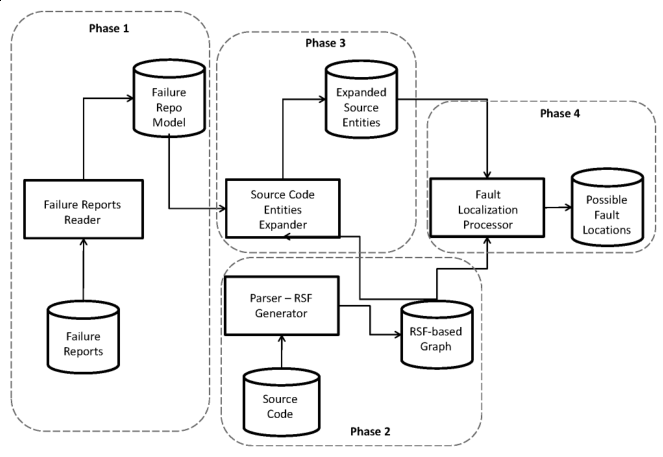
\includegraphics[width=500px]{../images/FaultPhases}

\hypertarget{development-objectives-0.75-page-max}{%
\section{\texorpdfstring{Development Objectives \emph{(0.75 page
max)}}{Development Objectives (0.75 page max)}}\label{development-objectives-0.75-page-max}}

\hypertarget{develop-a-complete-system-o1}{%
\subsubsection{Develop a complete system
(O1)}\label{develop-a-complete-system-o1}}

Since they are so many individual parts to the system required to run
the system, we wanted to combine scripts and Java code into an easy to
access complete system. Considering there were still some Python scripts
we did not get access to by the end of the project, it would be very
beneficial to have a complete system that is able to handle new
codebases and improve with new bug reports.

\hypertarget{be-able-to-integrate-with-a-github-based-workflow-o2}{%
\subsubsection{Be able to integrate with a GitHub based workflow
(O2)}\label{be-able-to-integrate-with-a-github-based-workflow-o2}}

We saw a great opportunity to integrate this system into GitHub's
system. Initially, the system was set up to read reports from BugZilla,
but we wanted to add the ability to integrate the system with GitHib's
issue tracker. This would entail fetching new issues as they are created
in a repo and processing them, pushing results back to the issue page so
the developers can get a head start, and allowing users to authenticate
using GitHub.

\hypertarget{operate-as-a-standalone-service-with-a-ui-o3}{%
\subsubsection{Operate as a standalone service with a UI
(O3)}\label{operate-as-a-standalone-service-with-a-ui-o3}}

The system initially was just run through a terminal, and because there
aren't too many options needed from the user, it would be beneficial to
create a system that can work independantly with an easy to use
interface. This would Work in a similar fashion to other CI tools, such
as Travis. We would also plan to give users the control to hook into any
of their repositories.

\hypertarget{system-requirements-2-pages-max}{%
\section{\texorpdfstring{System Requirements \emph{(2 pages
max)}}{System Requirements (2 pages max)}}\label{system-requirements-2-pages-max}}

\hypertarget{section-a-data-processing}{%
\subsubsection{Section A : Data
Processing}\label{section-a-data-processing}}

\begin{itemize}
\tightlist
\item
  \textbf{Feature 1:} Able to generate entity relationship rsf from
  codebase

  \begin{itemize}
  \tightlist
  \item
    FR 1: Pass code through cdif2rsf to generate rsf
  \item
    FR 2: Clean up incorrect entity and relationships
  \item
    FR 3: Store in accessible data storage for next step to use
  \end{itemize}
\item
  \textbf{Feature 2:} Able to generate set of keywords from bug
  description

  \begin{itemize}
  \tightlist
  \item
    FR 1: Compare each token to codebase to find valid functions
  \item
    FR 2: Expand initial token set by a factor of 3
  \item
    FR 3: Use NLP to determine question context
  \end{itemize}
\item
  \textbf{Feature 3:} Able to combine keywords and rsf into ranked
  outcomes

  \begin{itemize}
  \tightlist
  \item
    FR 1: Run LSI on each token and generate search space for each
  \item
    FR 2: Expand the search space for each result in FR 1
  \item
    FR 3: Find similarities between the initial token expansion and the
    final set of tokens
  \item
    FR 4: Apply ranking equation from research paper to come up with
    final outcome
  \end{itemize}
\end{itemize}

\hypertarget{section-b-front-end-user-interface}{%
\subsubsection{Section B : Front-End User
Interface}\label{section-b-front-end-user-interface}}

\begin{itemize}
\tightlist
\item
  \textbf{Feature 4:} User is able to scan and mark a new repository for
  processing

  \begin{itemize}
  \tightlist
  \item
    FR 1: Scan user's Github repos using Github's API
  \item
    FR 2: Allow the user to select ones they wish to run processing on
  \item
    FR 3: Remember which ones the user selected by storing on backend
  \end{itemize}
\item
  \textbf{Feature 5:} User is able to view the results of a new bug
  report's processing

  \begin{itemize}
  \tightlist
  \item
    FR 1: Monitor output from backend endpoints showing new results for
    user's repos
  \item
    FR 2: When a new bug report is created, and the processing finishes,
    show the output of that processing on a separate page
  \item
    FR 3: Allow the user to rerun processing on a specific bug report by
    sending a request to backend
  \end{itemize}
\item
  \textbf{Feature 6:} User is able to login using their Github
  credentials

  \begin{itemize}
  \tightlist
  \item
    FR 1: On first usage redirect user to Github's App authentication
    page
  \item
    FR 2: Ask backend to associate bug reports and repositories with
    this user
  \item
    FR 3: Redirect user to main UI
  \end{itemize}
\end{itemize}

\hypertarget{section-c-back-end-runtime-processing}{%
\subsubsection{Section C : Back-End Runtime
Processing}\label{section-c-back-end-runtime-processing}}

\begin{itemize}
\tightlist
\item
  \textbf{Feature 7:} Support front-end operations

  \begin{itemize}
  \tightlist
  \item
    FR 1: Allow registration using Github Auth
  \item
    FR 2: Allow retrieval of processing results for each bug report
  \item
    FR 3: Support re-running processing on a specific bug report
  \item
    FR 4: Create a API where the UI can fetch everything from
  \end{itemize}
\item
  \textbf{Feature 8:} Manage the automation of Data Processing (F1, F2,
  and F3)

  \begin{itemize}
  \tightlist
  \item
    FR 1: Automate RSF generation when a new repository is linked
  \item
    FR 2: Automate keyword generation when a new repository is linked
  \item
    FR 3: Continuously improve and modify RSF and keywords as code/bugs
    change
  \end{itemize}
\item
  \textbf{Feature 9:} Handle processing and evaluation when a new bug
  report comes in

  \begin{itemize}
  \tightlist
  \item
    FR 1: Monitor marked repositories for each registered user and
    trigger when new issue is filed
  \item
    FR 2: Run through automated ranking algorithm
  \item
    FR 3: Store result for later retrieval
  \item
    FR 4: Be able to connect to a repository and fetch an issue when it
    is posted
  \end{itemize}
\item
  \textbf{Feature 10:} Combine each element of data processing into the
  backend runtime

  \begin{itemize}
  \tightlist
  \item
    FR 1: Combine entity generation into token generation
  \item
    FR 2: Combine FR1 with RSF processing all into one unit
  \item
    FR 3: Move all functionality to an exposed part of the API
  \item
    FR 4: Create all endpoints for data processing functionality
  \end{itemize}
\end{itemize}

\hypertarget{development-strategy-2-pages-max}{%
\section{\texorpdfstring{Development Strategy \emph{(2 pages
max)}}{Development Strategy (2 pages max)}}\label{development-strategy-2-pages-max}}

Since this project had a lot of the main functionality already
implemented, we did not have many choices over what development tools
and languages to use. The majority of the project was written in Java,
with some separate Python scripts used for data manipulation at some of
the stages in the system. Including the development tools previously
mentioned, the following were also used in the system:

\hypertarget{technologies}{%
\subsubsection{Technologies}\label{technologies}}

\begin{itemize}
\tightlist
\item
  Kotlin
\item
  Python
\item
  Java
\item
  Javalin
\item
  MongoDB
\item
  Github Webhooks
\end{itemize}

\hypertarget{tools}{%
\subsubsection{Tools}\label{tools}}

\begin{itemize}
\tightlist
\item
  Intellij Idea
\item
  NeoVim
\item
  Robo3T
\item
  ngrok
\end{itemize}

\hypertarget{datasets}{%
\subsection{Datasets}\label{datasets}}

\begin{itemize}
\tightlist
\item
  BugZilla reports
\end{itemize}

\hypertarget{results-10-pages-max}{%
\section{\texorpdfstring{Results \emph{(10 pages
max)}}{Results (10 pages max)}}\label{results-10-pages-max}}

\hypertarget{buglocalization-project}{%
\subsubsection{BugLocalization Project}\label{buglocalization-project}}

\begin{itemize}
\tightlist
\item
  Restructured and cleaned up codebase
\item
  Reduced very large codebase to 10 files
\item
  Documented and made more readable for easier integration
\end{itemize}

\hypertarget{api}{%
\subsubsection{API}\label{api}}

\begin{itemize}
\tightlist
\item
  Able to monitor a GitHub repo for events
\item
  Detect new issues and add into a Mongo database
\item
  Able to start and end deployments on Pull Requests
\end{itemize}

\hypertarget{discussion-1.5-pages-max}{%
\section{\texorpdfstring{Discussion \emph{(1.5 pages
max)}}{Discussion (1.5 pages max)}}\label{discussion-1.5-pages-max}}

\hypertarget{threats-to-the-validity-of-the-results}{%
\subsubsection{Threats to the validity of the
results}\label{threats-to-the-validity-of-the-results}}

Due to the large amount of bug reports and the possibility of having
reports without enough details, the results are not guaranteed to find
where the fault occurs. The ranking used in the system is useful in
mitigating incorrect results, but does not gurantee that any of the
results will be useful in determining the cause of fault in the
software. A lot of other methods used to minimize the threats to
validity were already implemented in the project, but it was mentioned
that using different algorithms would allow us to compare the accuracy
of different methods.

\hypertarget{implications-of-the-results}{%
\subsubsection{Implications of the
results}\label{implications-of-the-results}}

One of the original goals of this project was to implement another
algorithm for determining the cause of fault to then use to compare the
validity of the results for both algorithms. The validity of the results
is important for a system like this because of how flexible it is for
testing on software projects. The system would be language agnostic and
allow the user to be able to accurately detect specific points of faults
in software projects that use multiple languages. This is much more
useful than traditional tools used for detecting issues in software and
would be applicable to any project, where those that have large projects
and/or use multiple languages would benefit the most. This system would
save software engineers lots of time and effort wasted on debugging
issues with software systems that don't provide enough information about
where a fault in the program occurs.

\hypertarget{limitations-of-the-results}{%
\subsubsection{Limitations of the
results}\label{limitations-of-the-results}}

The main limitation to this project is the complexity of being able to
detect a fault based on reports alone. When developing, users have many
methods of getting feedback through logs and error detection that are
not available to our system. The best way to remove this limitation
would be to get more details from failure reports, but unfortunately
there are not many alternatives that offer nearly as many reports as
BugZilla.

\hypertarget{conclusions-1-page-max}{%
\section{\texorpdfstring{Conclusions \emph{(1 page
max)}}{Conclusions (1 page max)}}\label{conclusions-1-page-max}}

Unfortunately, for our project we had some communication problems for a
large portion of the year. We ended up getting a late start to the
project and had to re-purpose the project after the second milestone.
Due to our late start and a couple missing scripts, we did not have
access to all parts of the system needed to create a complete system and
did not have enough time to create a standalone service with a UI. The
implications of creating a complete system would mean that the computer
running the system would have to be powerful enough to process all parts
of the analysis within a reasonable amount of time in order to be of use
to the programmer. Based on our testing with the components we had, we
believe that this would be achievable if given access to the remaining
parts of the program. We were able to refactor the code and greatly
improve the structure and readability. The main method contained too
much of the logic of the system, so modularizing the code and adding
comments made it much easier to understand for others who will look at
the code.

Completing O2 added the ability to connect to GitHub using their API and
get issues from their tracker. Since the biggest change to the existing
system is the report data used, the main structure of the system remains
the same while allowing it to be used in another useful domain. Using
this system in GitHub allows developers to easily discover faults in
their applications. The system is set to be run whenever an issue was
added by a user and would notify the repo owner.

\hypertarget{future-work-and-lessons-learnt-1-page-max}{%
\section{\texorpdfstring{Future Work and Lessons Learnt \emph{(1 page
max)}}{Future Work and Lessons Learnt (1 page max)}}\label{future-work-and-lessons-learnt-1-page-max}}

\hypertarget{future-work}{%
\subsubsection{Future work}\label{future-work}}

\begin{itemize}
\tightlist
\item
  Develop software to process issues incrementally into the
  BugLocalization
\item
  Integrate the BugLocalization project as part of the API and utilize
  its full power
\item
  Make a web UI similar to Travis to display results
\end{itemize}

\hypertarget{lessons-learnt}{%
\subsubsection{Lessons learnt}\label{lessons-learnt}}

\begin{itemize}
\tightlist
\item
  Develop consistent communication plan with stakeholders
\end{itemize}

\bibliography{}

%----------------------------------------------------------------------------------------

\end{document}
